

\chapter{Appendix}
\label{Appendix}

\section{Suplementary figures}
\label{Suplementary figures}

\begin{figure}[htbp]
  \centering
  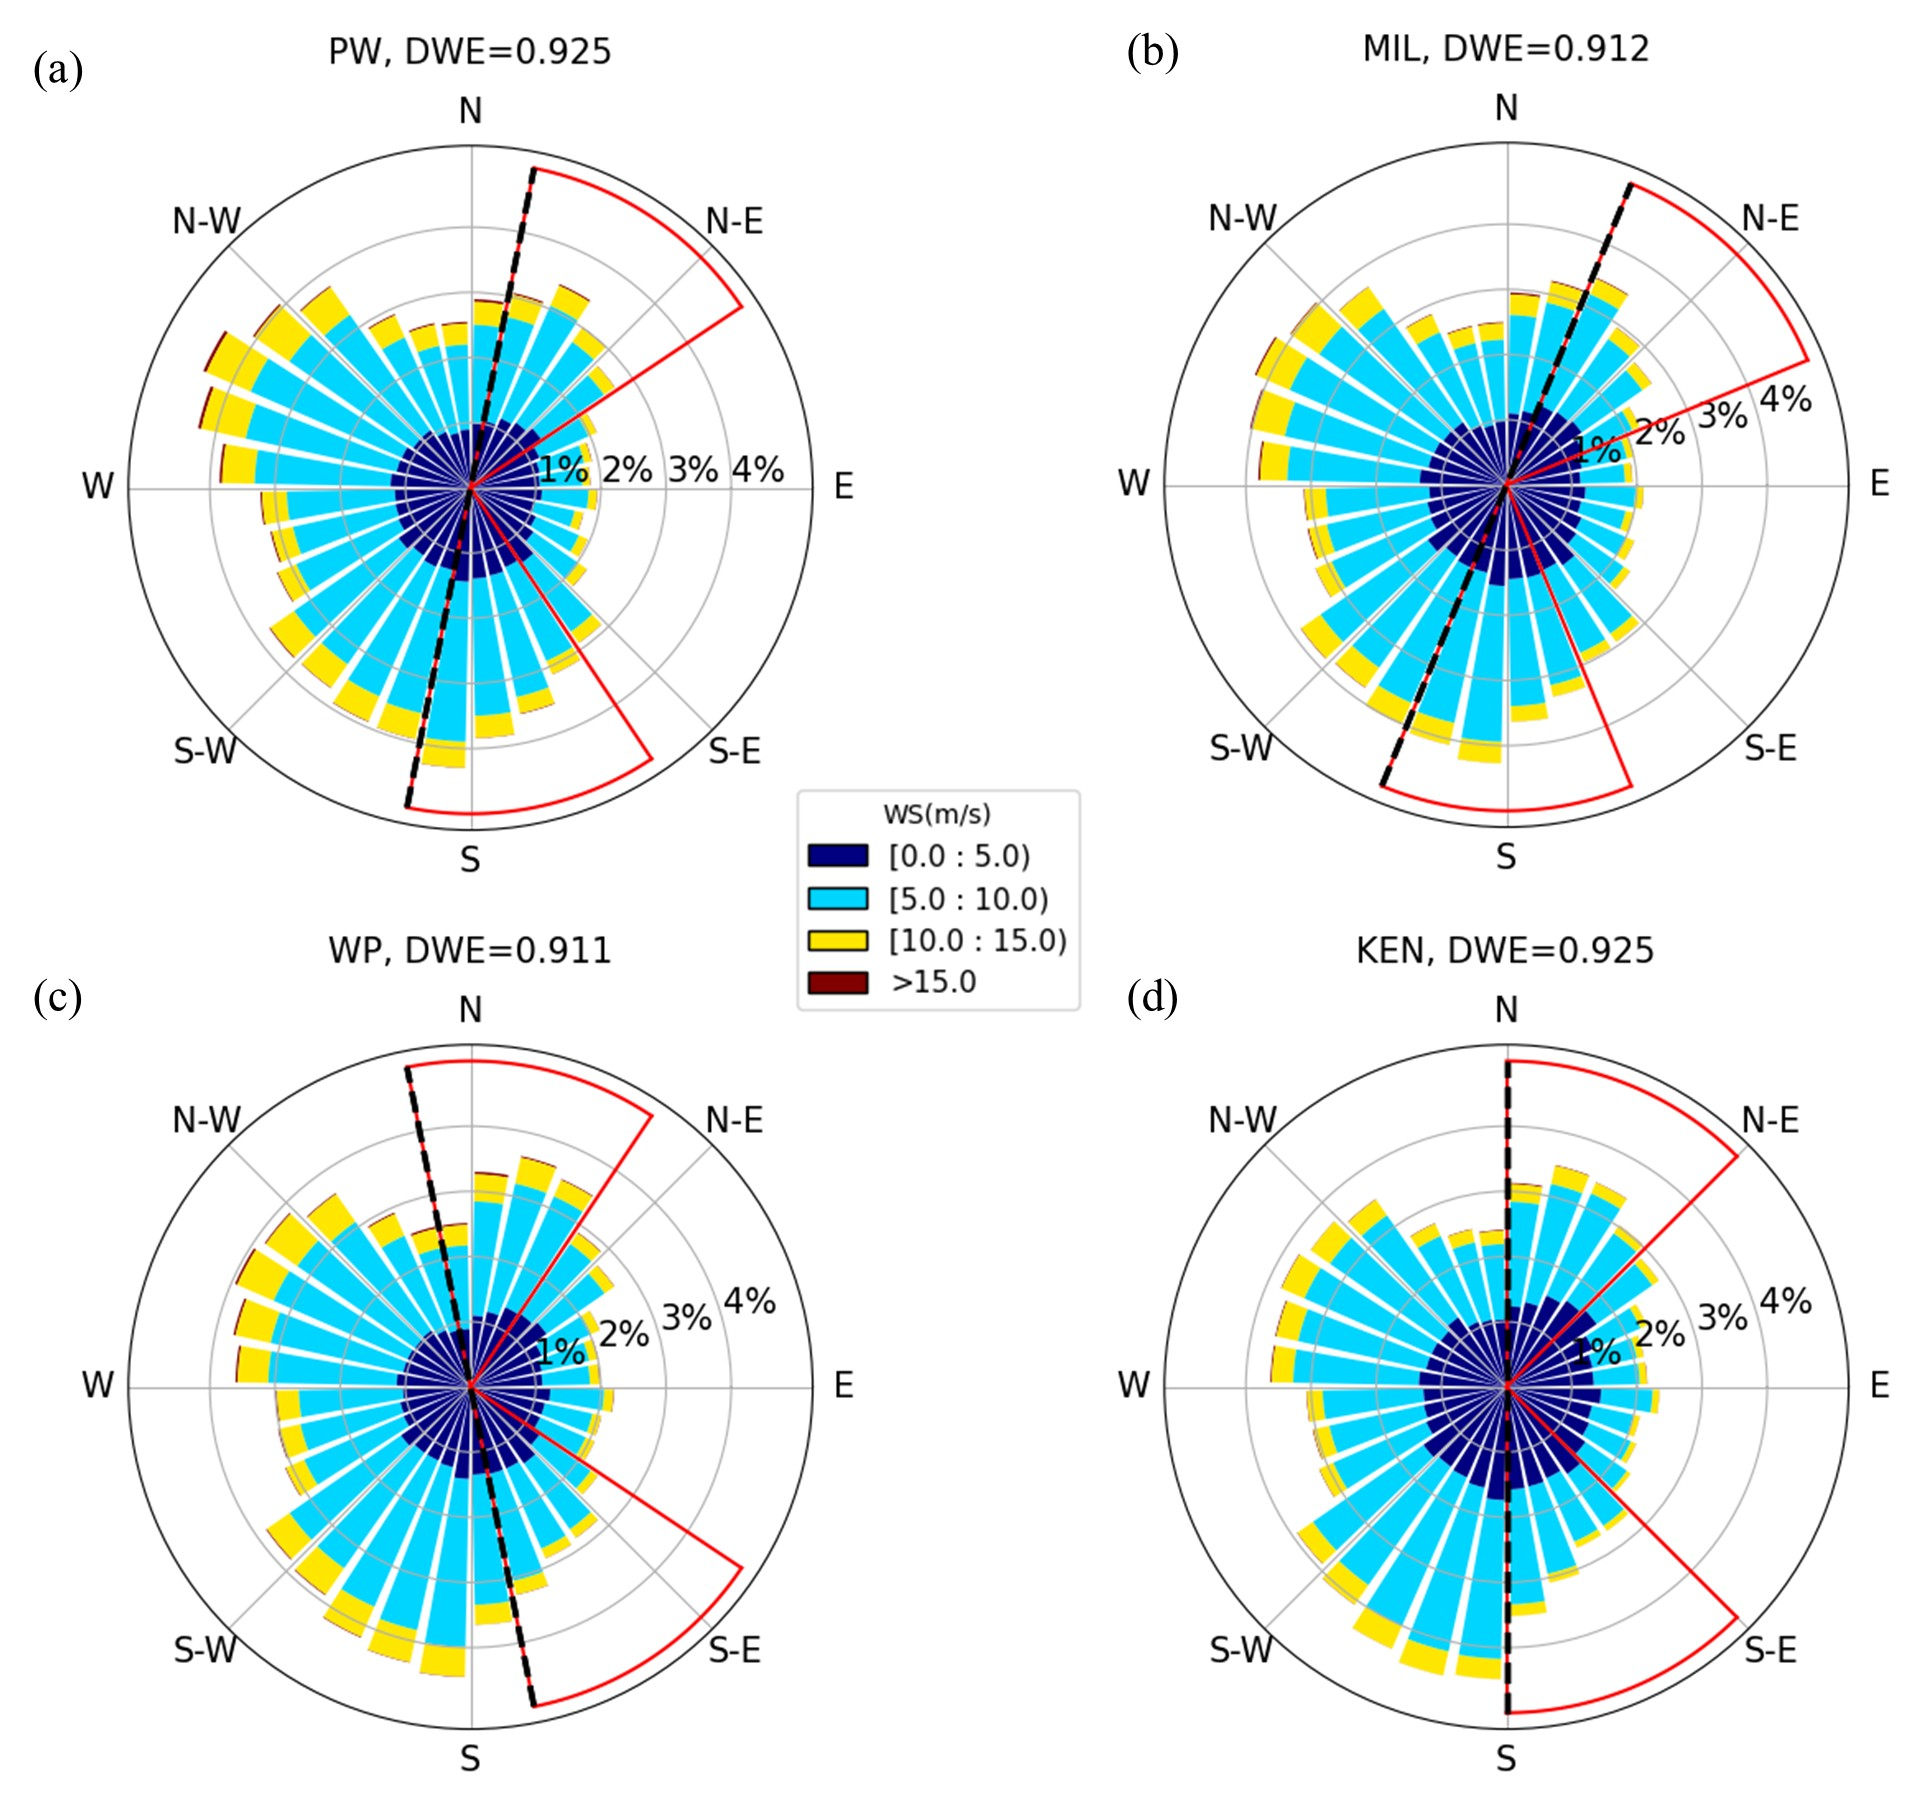
\includegraphics[width=0.8\textwidth]{appendix/resources/figure3-1a.jpg}
  \caption{Wind rose maps and DWE at 4 selected locations. (a) PW-Port Washington, (b) MIL-Milwaukee Harbor, (c) WP-Wind Point, and (d) KEN-Kenosha Harbor with their directional wave (wind) entropy.}
  \label{fig:fig3.1a}
\end{figure}

\begin{figure}[htbp]
  \centering
  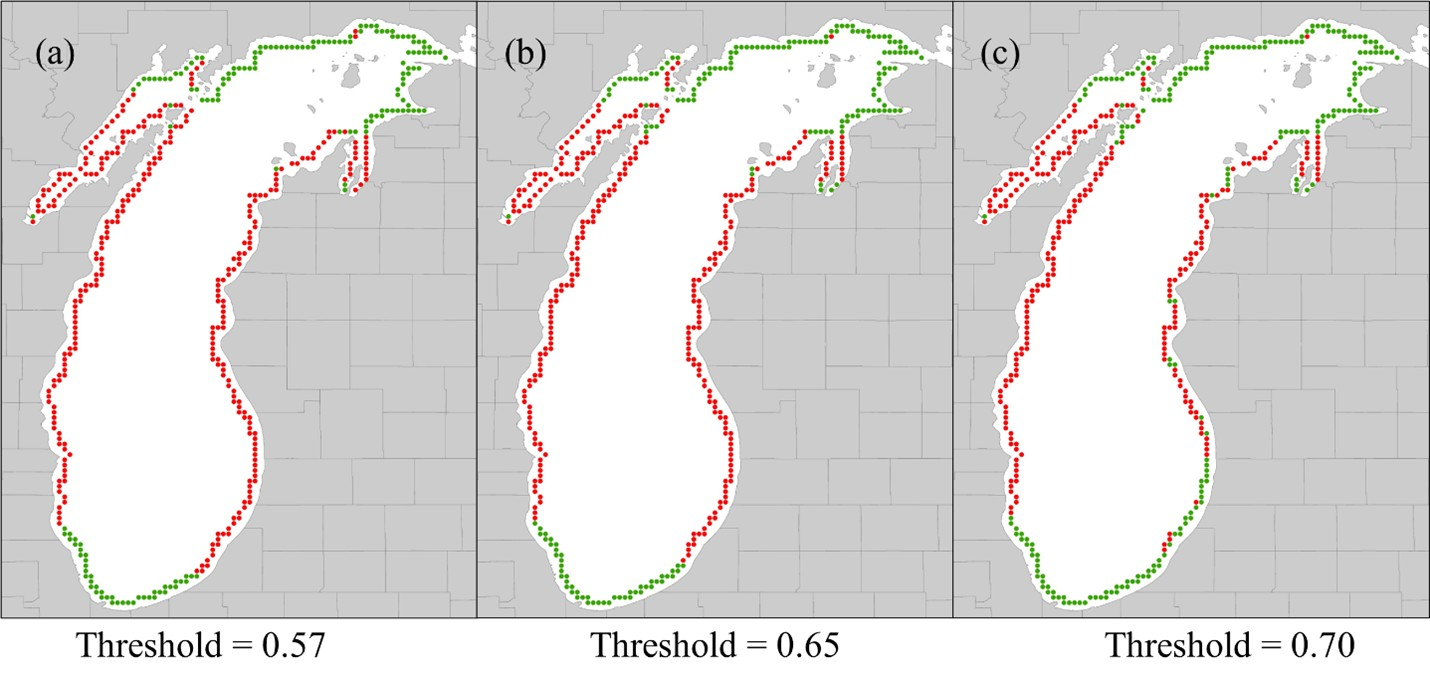
\includegraphics[width=0.8\textwidth]{appendix/resources/figure3-2a.jpg}
  \caption{Wave directionality in Lake Michigan for different DWE thresholds. Wave directionality (red dots are bi-directional and green dots are uni-directional) under three different thresholds: (a) 0.57 (b) 0.65 (c) 0.70.}
  \label{fig:fig3.2a}
\end{figure}

\begin{figure}[htbp]
  \centering
  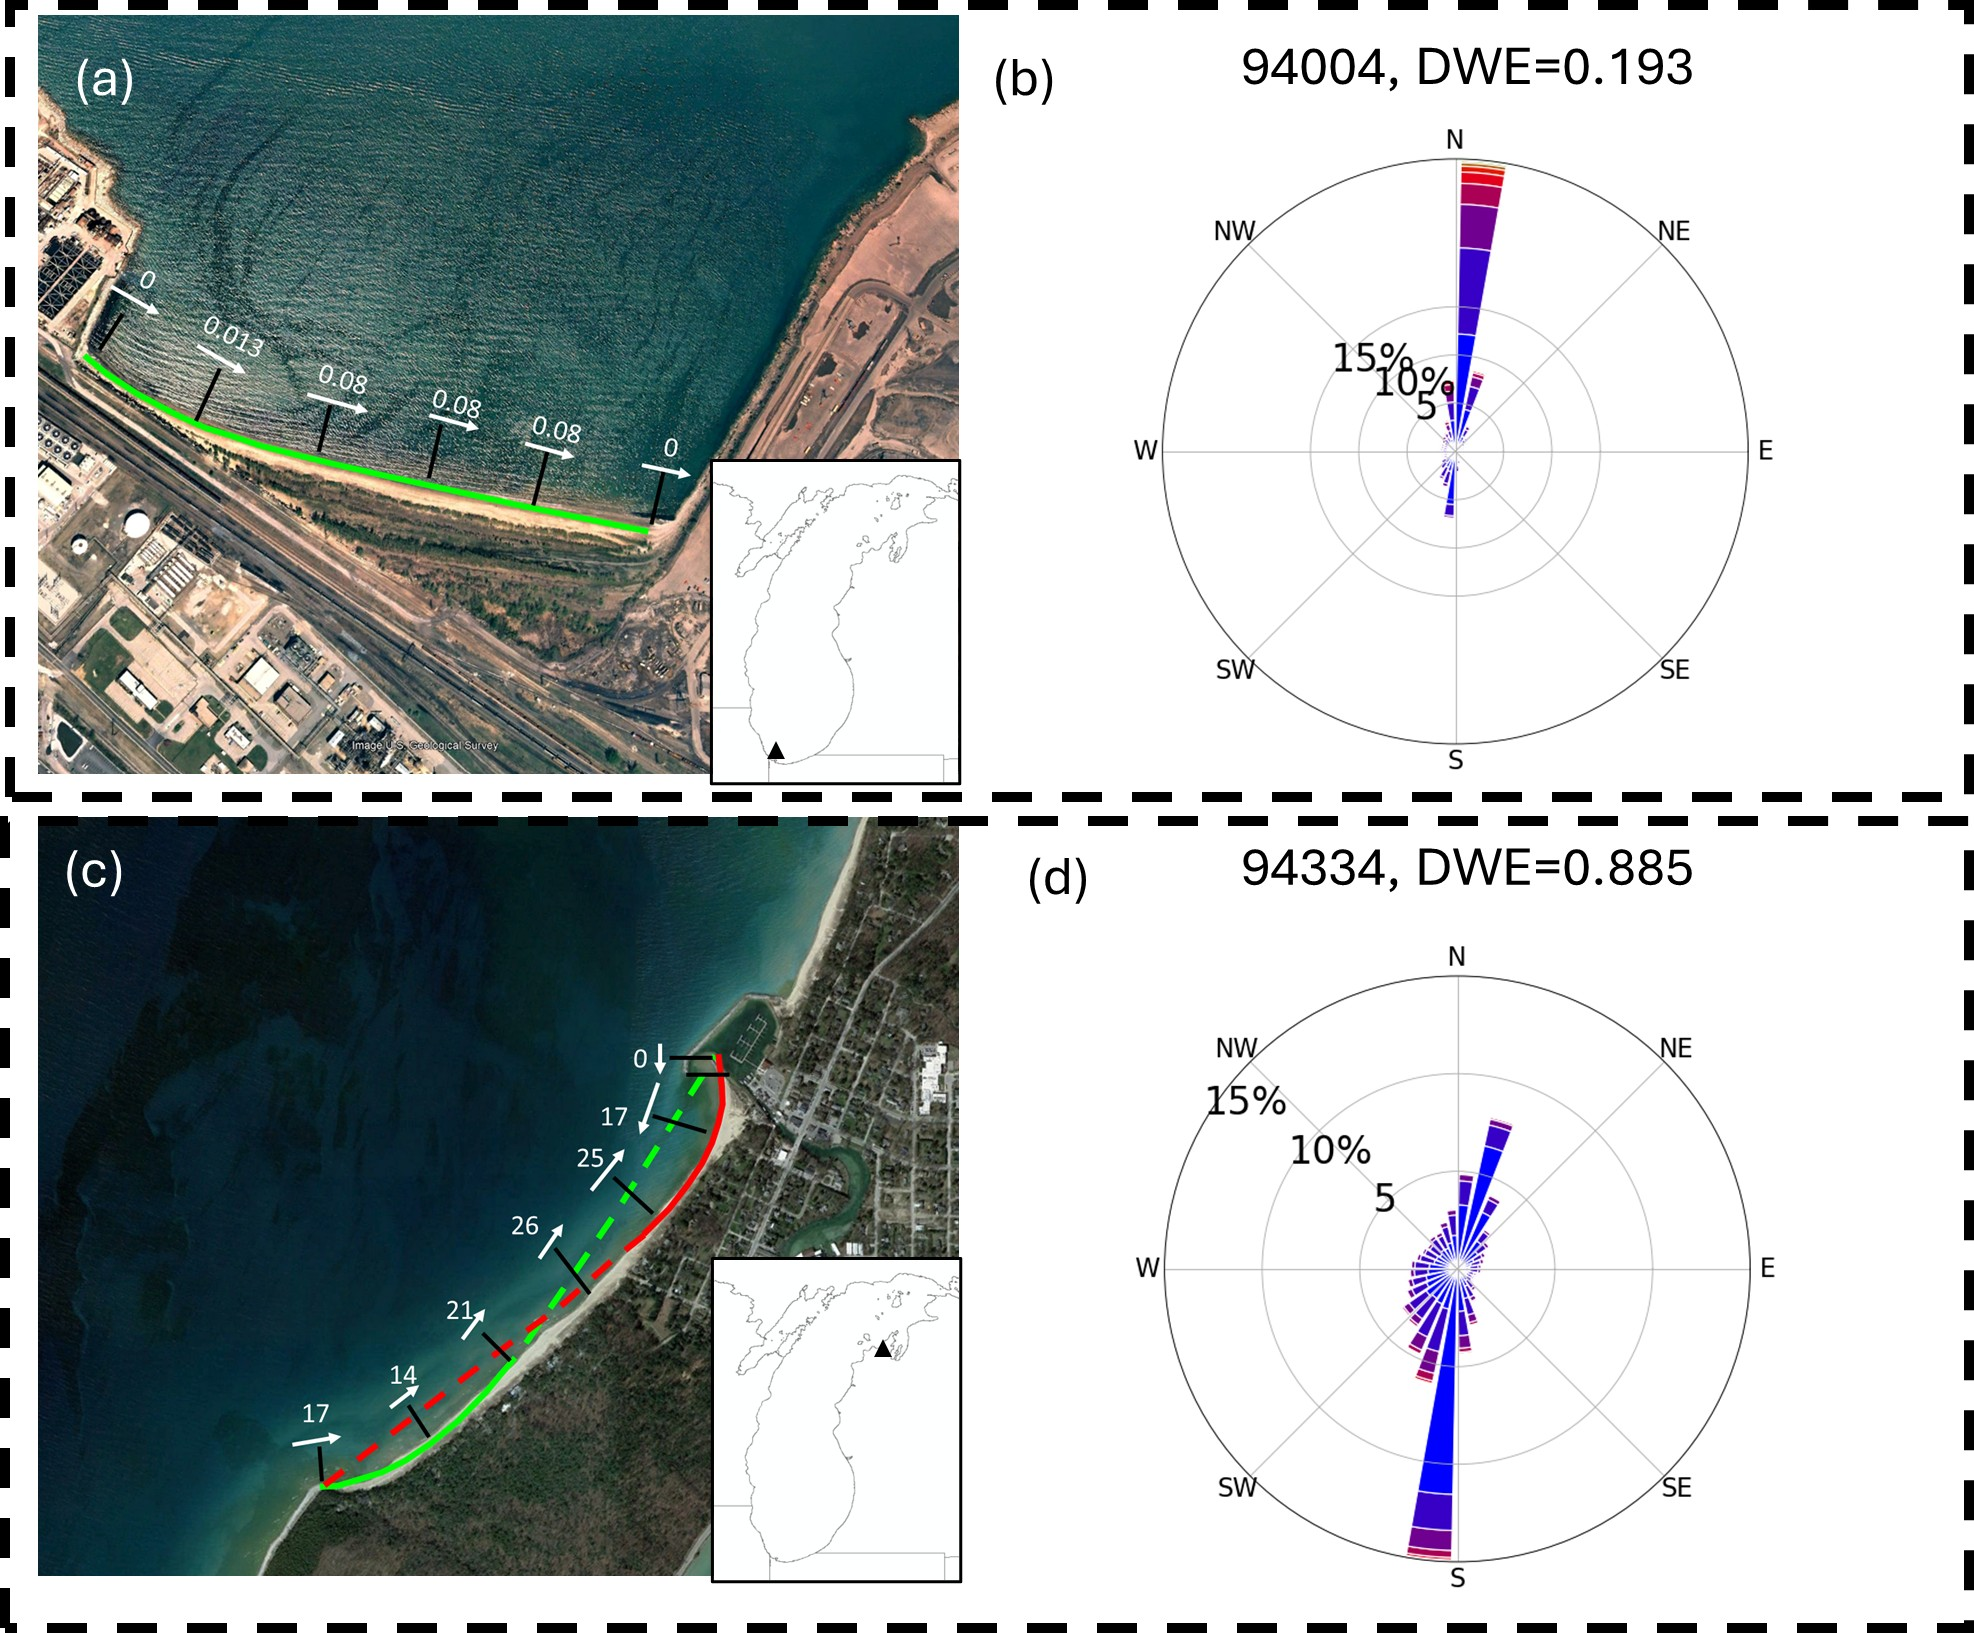
\includegraphics[width=0.8\textwidth]{appendix/resources/figure3-3a.jpg}
  \caption{Wave directionality in Lake Michigan for different DWE thresholds. Wave directionality (red dots are bi-directional and green dots are uni-directional) under three different thresholds: (a) 0.57 (b) 0.65 (c) 0.70. The unit of LST rate is cubic meter per day.}
  \label{fig:fig3.3a}
\end{figure}

\section{Suplementary tables}
\label{Suplementary tables}
\sisetup{scientific-notation = true, output-exponent-marker = \mathrm{e}}
\begin{table}[htbp]
\centering
\caption{Coastal vulnerability indicator in Oak Creek Beach}
\label{tab:oak_indicator}
\footnotesize
\setlength{\tabcolsep}{2.5pt}% tighter columns
\renewcommand{\arraystretch}{0.95}% tighter rows
\begin{tabular}{@{}p{0.49\linewidth}@{} p{0.49\linewidth}@{}}
\begin{minipage}[t]{\linewidth}
\textbf{Year 2008}\\[-2pt]
\begin{tabular}{r S[table-format=1.3e-2] S[table-format=1.3] S[table-format=1.3] S[table-format=3.3] S[table-format=5.3]}
\toprule
id & {BFI} & {whdi} & {wsi} & {lri} & {SBI} \\
\midrule
0 & 1.602e-04 & 0.147 & 0.747 & 49.093 & 163.481 \\
1 & 1.491e-04 & 0.745 & 0.541 & 46.059 & 1943.461 \\
2 & 9.177e-05 & 0.782 & 0.489 & 70.100 & 2627.785 \\
3 & 3.536e-05 & 0.782 & 0.486 & 182.000 & 2597.358 \\
4 & 1.443e-05 & 0.818 & 0.419 & 393.198 & 4165.131 \\
5 & 1.832e-04 & 0.815 & 0.427 & 28.943 & 3876.458 \\
6 & 1.447e-04 & 0.821 & 0.405 & 41.049 & 4656.092 \\
7 & 6.293e-05 & 0.827 & 0.383 & 113.458 & 5786.886 \\
8 & 7.336e-05 & 0.831 & 0.358 & 88.057 & 7338.612 \\
\bottomrule
\end{tabular}

\vspace{4pt}
\textbf{Year 2013}\\[-2pt]
\begin{tabular}{r S[table-format=1.3e-2] S[table-format=1.3] S[table-format=1.3] S[table-format=3.3] S[table-format=5.3]}
\toprule
id & {BFI} & {whdi} & {wsi} & {lri} & {SBI} \\
\midrule
0 & 1.741e-04 & 0.683 & 0.599 & 49.467 & 2304.561 \\
1 & 1.437e-04 & 0.706 & 0.584 & 46.202 & 2630.877 \\
2 & 8.905e-05 & 0.796 & 0.481 & 70.610 & 4841.806 \\
3 & 3.277e-05 & 0.797 & 0.480 & 183.395 & 4873.920 \\
4 & 1.325e-05 & 0.833 & 0.440 & 395.430 & 6453.914 \\
5 & 1.647e-04 & 0.842 & 0.427 & 29.194 & 7146.901 \\
6 & 1.218e-04 & 0.839 & 0.434 & 41.249 & 6767.752 \\
7 & 4.829e-05 & 0.850 & 0.397 & 114.513 & 9595.957 \\
8 & 5.387e-05 & 0.851 & 0.389 & 88.562 & 10189.244 \\
\bottomrule
\end{tabular}
\end{minipage}
 & 
\begin{minipage}[t]{\linewidth}
\textbf{Year 2015}\\[-2pt]
\begin{tabular}{r S[table-format=1.3e-2] S[table-format=1.3] S[table-format=1.3] S[table-format=3.3] S[table-format=5.3]}
\toprule
id & {BFI} & {whdi} & {wsi} & {lri} & {SBI} \\
\midrule
0 & 2.173e-04 & 0.524 & 0.866 & 49.327 & 2204.725 \\
1 & 1.770e-04 & 0.748 & 0.761 & 46.322 & 4497.898 \\
2 & 1.092e-04 & 0.795 & 0.708 & 70.633 & 5924.765 \\
3 & 3.829e-05 & 0.785 & 0.718 & 183.277 & 5662.569 \\
4 & 1.453e-05 & 0.817 & 0.678 & 395.469 & 7069.057 \\
5 & 1.825e-04 & 0.803 & 0.698 & 29.052 & 6186.392 \\
6 & 1.355e-04 & 0.817 & 0.656 & 41.367 & 7907.233 \\
7 & 5.229e-05 & 0.811 & 0.652 & 114.059 & 8109.591 \\
8 & 6.113e-05 & 0.814 & 0.644 & 88.142 & 8278.407 \\
\bottomrule
\end{tabular}

\vspace{4pt}
\textbf{Year 2018}\\[-2pt]
\begin{tabular}{r S[table-format=1.3e-2] S[table-format=1.3] S[table-format=1.3] S[table-format=3.3] S[table-format=5.3]}
\toprule
id & {BFI} & {whdi} & {wsi} & {lri} & {SBI} \\
\midrule
0 & 4.045e-04 & 0.786 & 0.663 & 49.606 & 4334.829 \\
1 & 2.282e-04 & 0.826 & 0.591 & 46.576 & 6889.294 \\
2 & 1.402e-04 & 0.824 & 0.601 & 70.584 & 6498.832 \\
3 & 4.467e-05 & 0.844 & 0.520 & 185.187 & 11572.806 \\
4 & 1.535e-05 & 0.844 & 0.527 & 397.100 & 10882.720 \\
5 & 1.849e-04 & 0.845 & 0.518 & 29.314 & 11786.208 \\
6 & 1.314e-04 & 0.846 & 0.497 & 41.650 & 13966.062 \\
7 & 4.968e-05 & 0.845 & 0.502 & 114.562 & 13491.119 \\
8 & 6.420e-05 & 0.845 & 0.517 & 88.103 & 11843.981 \\
\bottomrule
\end{tabular}
\end{minipage}\\
\end{tabular}
\end{table}
% Requires: \usepackage{booktabs,siunitx}
\sisetup{scientific-notation = true, output-exponent-marker = \mathrm{e}}
\begin{table}[htbp]
\centering
\caption{Coastal vulnerability indicator in Whitting Park Beach}
\label{tab:whitting_indicator}
\footnotesize
\setlength{\tabcolsep}{2.5pt}
\renewcommand{\arraystretch}{0.95}
\begin{tabular}{@{}p{0.49\linewidth}@{} p{0.49\linewidth}@{}}
\begin{minipage}[t]{\linewidth}
\textbf{Year 2010}\\[-2pt]
\begin{tabular}{r S[table-format=1.3e-2] S[table-format=1.3] S[table-format=1.3] S[table-format=3.3] S[table-format=5.3]}
\toprule
id & {BFI} & {whdi} & {wsi} & {lri} & {SBI} \\
\midrule
0 & 4.243e-04 & 0.810 & 0.235 & 70.652 & 11963.609 \\
1 & 2.808e-04 & 0.768 & 0.224 & 80.274 & 8452.093 \\
2 & 1.854e-04 & 0.712 & 0.222 & 65.942 & 5634.264 \\
3 & 7.097e-05 & 0.628 & 0.221 & 99.590 & 3595.784 \\
4 & 6.794e-05 & 0.578 & 0.221 & 72.415 & 3058.351 \\
5 & 4.531e-05 & 0.468 & 0.220 & 80.613 & 1561.635 \\
6 & 3.880e-05 & 0.058 & 0.220 & 74.257 & 202.720 \\
7 & 4.420e-05 & 0.578 & 0.221 & 59.271 & 3205.233 \\
\bottomrule
\end{tabular}

\vspace{4pt}
\textbf{Year 2012}\\[-2pt]
\begin{tabular}{r S[table-format=1.3e-2] S[table-format=1.3] S[table-format=1.3] S[table-format=3.3] S[table-format=5.3]}
\toprule
id & {BFI} & {whdi} & {wsi} & {lri} & {SBI} \\
\midrule
0 & 2.555e-04 & 0.823 & 0.416 & 71.099 & 8353.144 \\
1 & 2.052e-04 & 0.756 & 0.408 & 80.704 & 5955.700 \\
2 & 1.457e-04 & 0.553 & 0.410 & 66.298 & 3381.609 \\
3 & 6.079e-05 & 0.027 & 0.411 & 100.145 & 967.013 \\
4 & 5.974e-05 & 0.026 & 0.412 & 72.808 & 1175.395 \\
5 & 4.067e-05 & 0.125 & 0.412 & 81.055 & 262.940 \\
6 & 3.627e-05 & 0.053 & 0.410 & 74.613 & 541.830 \\
7 & 4.185e-05 & 0.052 & 0.409 & 59.608 & 361.943 \\
\bottomrule
\end{tabular}

\vspace{4pt}
\textbf{Year 2014}\\[-2pt]
\begin{tabular}{r S[table-format=1.3e-2] S[table-format=1.3] S[table-format=1.3] S[table-format=3.3] S[table-format=5.3]}
\toprule
id & {BFI} & {whdi} & {wsi} & {lri} & {SBI} \\
\midrule
0 & 3.547e-04 & 0.789 & 0.458 & 70.816 & 10473.172 \\
1 & 2.687e-04 & 0.724 & 0.462 & 80.415 & 6507.299 \\
2 & 1.622e-04 & 0.627 & 0.467 & 66.050 & 3434.631 \\
3 & 6.489e-05 & 0.523 & 0.471 & 99.714 & 2226.910 \\
4 & 6.452e-05 & 0.525 & 0.469 & 72.500 & 1925.151 \\
5 & 4.386e-05 & 0.166 & 0.470 & 80.723 & 59.213 \\
6 & 3.837e-05 & 0.525 & 0.469 & 74.282 & 1863.216 \\
7 & 4.409e-05 & 1.000 & 0.467 & 59.445 & 7204.682 \\
\bottomrule
\end{tabular}
\end{minipage}
 & 
\begin{minipage}[t]{\linewidth}
\textbf{Year 2016}\\[-2pt]
\begin{tabular}{r S[table-format=1.3e-2] S[table-format=1.3] S[table-format=1.3] S[table-format=3.3] S[table-format=5.3]}
\toprule
id & {BFI} & {whdi} & {wsi} & {lri} & {SBI} \\
\midrule
0 & 5.788e-04 & 0.789 & 0.356 & 71.039 & 13004.747 \\
1 & 3.695e-04 & 0.695 & 0.344 & 80.708 & 7836.622 \\
2 & 2.001e-04 & 0.578 & 0.348 & 66.274 & 4777.970 \\
3 & 7.551e-05 & 0.548 & 0.349 & 100.033 & 4349.886 \\
4 & 7.185e-05 & 0.370 & 0.352 & 72.771 & 1612.956 \\
5 & 4.688e-05 & 0.089 & 0.355 & 81.023 & 235.856 \\
6 & 3.870e-05 & 0.749 & 0.365 & 74.660 & 4805.265 \\
7 & 4.233e-05 & 0.801 & 0.367 & 59.649 & 5531.369 \\
\bottomrule
\end{tabular}

\vspace{4pt}
\textbf{Year 2018}\\[-2pt]
\begin{tabular}{r S[table-format=1.3e-2] S[table-format=1.3] S[table-format=1.3] S[table-format=3.3] S[table-format=5.3]}
\toprule
id & {BFI} & {whdi} & {wsi} & {lri} & {SBI} \\
\midrule
0 & 1.150e-03 & 0.741 & 0.446 & 77.079 & 12941.043 \\
1 & 6.658e-04 & 0.617 & 0.439 & 74.730 & 8322.721 \\
2 & 1.985e-04 & 0.437 & 0.434 & 72.896 & 2552.905 \\
3 & 8.433e-05 & 0.402 & 0.435 & 94.578 & 2223.274 \\
4 & 7.123e-05 & 0.139 & 0.434 & 75.301 & 787.034 \\
5 & 4.735e-05 & 0.469 & 0.432 & 77.099 & 5302.978 \\
6 & 3.689e-05 & 0.767 & 0.433 & 75.476 & 7437.827 \\
7 & 4.277e-05 & 0.837 & 0.434 & 57.554 & 7932.480 \\
\bottomrule
\end{tabular}
\end{minipage}\\
\end{tabular}
\end{table}